\documentclass[10pt]{article}
\usepackage[english]{babel}
\usepackage{../../../meta-inf/lib/naproche}
\usepackage{amssymb}
\usepackage{mathtools} % for \coloneq

\usepackage{stex-highlighting}
\providebool{emph} % "\newbool{emph}" does not work...
\setbool{emph}{false}
\colorlet{emphcolor}{violet}
\let\oldemph\emph
\renewcommand\emph[1]{\setbool{emph}{true}\ifbool{forthel}{\textcolor{emphcolor}{\itshape#1}}{\oldemph{#1}}\setbool{emph}{false}}
\renewcommand{\varemph}[1]{\ifbool{emph}{\textcolor{emphcolor}{#1}}{\textcolor{black}{#1}}}

\usepackage[right=6cm,left=3cm,bottom=3cm,marginparwidth=5cm]{geometry}

\usepackage{fancyhdr}
\renewcommand{\sectionmark}[1]{\markboth{#1}{}} 
\def\libarchive{}
\pagestyle{fancy}
\fancyhead[L]{\libarchive}
\fancyhead[C]{\nouppercase\leftmark}  % section title
\fancyhead[R]{\thepage}               % page number
\fancyfoot[C]{}                       % No page number in footer

\usepackage[nobottomtitles]{titlesec}
\titlespacing*{\section}{0pt}{30pt}{0pt}
\titlespacing*{\subsection}{0pt}{30pt}{0pt}
\titlespacing*{\subsubsection}{0pt}{30pt}{0pt}

\documentclass[12pt,oneside]{book}

\usepackage[foundations]{../../lib/tex/naproche}
\usepackage{../../lib/tex/libraries}
\usepackage{graphicx}
\usepackage{float}
\usepackage{caption}
\usepackage{footnote}

\makesavenoteenv{tabular} % Make footnotes work in tabular environments


\title{Foundations of Mathematics}
\author{Marcel Schütz}
\date{2022}

\begin{document}
  \maketitle

  \tableofcontents

  \begin{figure}[H]
    \centering
    \fbox{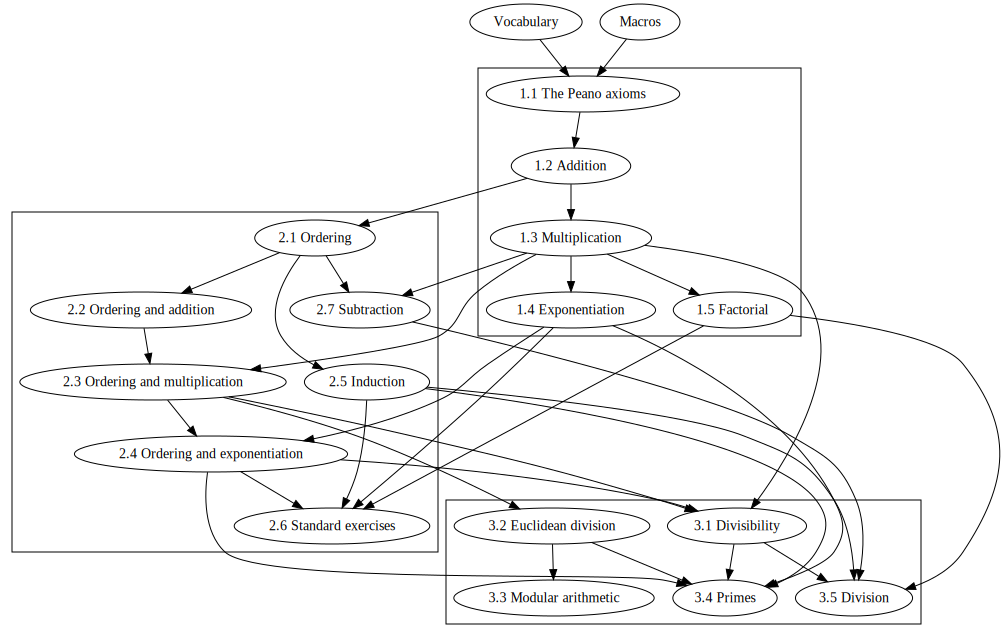
\includegraphics[width=0.9\linewidth]{./dependency-graph/graph.png}}
    \caption*{Interdependencies of the chapters}
  \end{figure}


  \section*{Introduction}

  This is a library providing a foundation of mathematics based on a
  Kelley-Morse like class theory with urelements.
  It introduces common operations on classes like unions or intersections
  (\cref{chapter:classes}) together with detailed proofs of their algebraic
  properties (\cref{chapter:computation-laws-for-classes}), the symmetric
  difference of two classes (\cref{chapter:symmetric-difference}) and the
  notions of ordered pairs and Cartesian products
  (\cref{chapter:pairs-and-products}) as well as proofs of the algebraic
  properties of the latter (\cref{chapter:computation-laws-for-products}).
  Moreover, it provides common operations on maps (\cref{chapter:maps}), various
  properties of images and preimages (\cref{chapter:image-and-preimage}) and the
  notions of injectivity, surjectivity, bijectivity
  (\cref{chapter:injections-surjections-bijections}) and invertibility of maps
  (\cref{chapter:invertible-maps}).
  The library provides an axiom system characterizing sets (\cref{chapter:sets})
  and, furthermore, it covers the notions of binary relations
  (\cref{chapter:binary-relations}), fixed-points of subset preserving maps
  (\cref{chapter:fixed-points}), including and equinumerosity
  (\cref{chapter:equinumerosity}).

  As two famous results it includes the Knaster-Tarski fixed point theorem
  (\cref{FOUNDATIONS_12_8420450166112256}) and the Cantor-Schröder-Bernstein
  theorem (\cref{FOUNDATIONS_13_1913663275401216}).

  \paragraph*{Usage.}
  At the very beginning of each chapter you can find the name of its source
  file, e.g. \path{foundations/sections/01_classes.ftl.tex} for
  \cref{chapter:classes}. This filename can be used to import the chapter via
  \Naproche's \texttt{readtex} instruction to another ForTheL text, e.g.:
  \begin{center}
    \verb`[readtex \path{foundations/sections/01_classes.ftl.tex}]`
  \end{center}

  \paragraph*{Checking times.}
  The checking times for each of the chapters may vary from computer to
  computer, but on mid-range hardware they are likely to be similar to those
  given in table below:

  \begin{center}
    \begin{tabular}{c|c|c}

      & \multicolumn{2}{c}{\textbf{Checking time}}
      \\
      \textbf{Chapter}
      & \textbf{without dependencies}     & \textbf{with dependencies}
      \\ \hline
      \ref{chapter:classes}
      & 00:04 min                         & 00:04 min
      \\
      \ref{chapter:computation-laws-for-classes}
      & 00:12 min                         & 00:16 min
      \\
      \ref{chapter:symmetric-difference}
      & 00:32 min                         & 00:48 min
      \\
      \ref{chapter:pairs-and-products}
      & 00:08 min                         & 00:12 min
      \\
      \ref{chapter:computation-laws-for-products}
      & 01:36 min                         & 01:56 min
      \\
      \ref{chapter:maps}
      & 01:13 min                         & 01:25 min
      \\
      \ref{chapter:image-and-preimage}
      & 01:28 min                         & 02:53 min
      \\
      \ref{chapter:injections-surjections-bijections}
      & 00:38 min                         & 02:03 min
      \\
      \ref{chapter:invertible-maps}
      & 02:20 min                         & 04:23 min
      \\
      \ref{chapter:sets}
      & 02:17 min                         & 06:40 min
      \\
      \ref{chapter:binary-relations}
      & 00:14 min                         & 06:54 min
      \\
      \ref{chapter:fixed-points}
      & 00:33 min                         & 07:13 min
      \\
      \ref{chapter:equinumerosity}
      & 01:48 min                         & 09:01 min
    \end{tabular}
  \end{center}


  \subfile{sections/01_classes.ftl.tex}
  \subfile{sections/02_computation-laws-for-classes.ftl.tex}
  \subfile{sections/03_symmetric-difference.ftl.tex}
  \subfile{sections/04_pairs-and-products.ftl.tex}
  \subfile{sections/05_computation-laws-for-products.ftl.tex}
  \subfile{sections/06_maps.ftl.tex}
  \subfile{sections/07_image-and-preimage.ftl.tex}
  \subfile{sections/08_injections-surjections-bijections.ftl.tex}
  \subfile{sections/09_invertible-maps.ftl.tex}
  \subfile{sections/10_sets.ftl.tex}
  \subfile{sections/11_binary-relations.ftl.tex}
  \subfile{sections/12_fixed-points.ftl.tex}
  \subfile{sections/13_equinumerosity.ftl.tex}
\end{document}

\usepackage{amssymb}

\newcommand{\Nat}{\mathbb{N}}
\newcommand{\Prime}{\mathbb{P}}
\renewcommand{\succ}{\textrm{succ}}
\newcommand{\pred}{\textrm{pred}}
\newcommand{\add}{\textrm{add}}
\newcommand{\mul}{\textrm{mul}}
\renewcommand{\exp}{\textrm{exp}}
\newcommand{\fac}{\textrm{fac}}
\renewcommand{\div}{\mathop{\textrm{div}}}
\renewcommand{\mod}{\mathop{\textrm{mod}}}

\begin{document}
  \begin{imports}
    \begin{forthel}
      %[prove off][check off]
      [readtex \path{libraries/source/foundations/segments-of-natural-numbers.ftl.tex}]
      [readtex \path{libraries/source/foundations/equinumerosity.ftl.tex}]
      %[prove on][check on]
    \end{forthel}
  \end{imports}


  \section*{Finite and Infinite Classes}

  \subsection*{Finite Classes}

  \begin{forthel}
    \begin{definition}[id=FOUNDATIONS_14_3512046897512410,printid]
      Let $X$ be a class and $n$ be a natural number.
      $X$ has $n$ elements iff $X$ is equinumerous to $\{ 1, \dots, n \}$.
    \end{definition}
  \end{forthel}

  \begin{forthel}
    \begin{definition}[id=FOUNDATIONS_14_3694156977274880,printid]
      Let $X$ be a class.
      $X$ is finite iff there exists a natural number $n$ such that $X$ has $n$ elements.
    \end{definition}
  \end{forthel}

  \begin{forthel}
    \begin{proposition}[id=FOUNDATIONS_14_3929085203972096,printid]
      Let $X, Y$ be classes.
      If $X$ is finite and $Y$ is equinumerous to $X$ then $Y$ is finite.
    \end{proposition}
    \begin{proof}
      Assume that $X$ is finite and $Y$ is equinumerous to $X$.
      Take a natural number $n$ and a bijection $f$ between $\{ 1, \dots, n \}$ and $X$ and a bijection $g$ between $X$ and $Y$.
      Then $g \circ f$ is a bijection between $\{ 1, \dots, n \}$ and $Y$ (by \printref{FOUNDATIONS_08_6435206693126144}).
      Indeed $X, Y$ are classes.
      Hence $Y$ is finite.
    \end{proof}
  \end{forthel}

  \begin{forthel}
    \begin{proposition}[id=FOUNDATIONS_14_5132547854597502,printid]
      Let $X$ be a class.
      $X$ has $0$ elements iff $X = \emptyset$.
    \end{proposition}
  \end{forthel}

  \begin{forthel}
    \begin{proposition}[id=FOUNDATIONS_14_6812054297034125,printid]
      Let $X$ be a class.
      $X$ has $1$ element iff $X = \set{a}$ for some object $a$.
    \end{proposition}
    \begin{proof}
      Case $X$ has $1$ element.
        Take a bijection $f$ between $\{ 1, \dots, 1 \}$ and $X$.
        We have $\{ 1, \dots, 1 \} = \set{1}$.
        Hence $X = \set{f(1)}$.
      End.

      Case $X = \set{a}$ for some object $a$.
        Consider an object $a$ such that $X = \set{a}$.
        Define $f(x) = 1$ for $x \in \set{a}$.
      Then $f$ is a bijection between $\set{a}$ and $\{ 1, \dots, 1 \}$.
      End.
    \end{proof}
  \end{forthel}

  \begin{forthel}
    \begin{proposition}[id=FOUNDATIONS_14_3468912675458910,printid]
      Let $X$ be a class.
      $X$ has $2$ elements iff $X = \set{a, b}$ for some distinct objects $a, b$.
    \end{proposition}
    \begin{proof}
      Case $X$ has $2$ elements.
        Take a bijection $f$ between $\{ 1, \dots, 2 \}$ and $X$.
        We have $\{ 1, \dots, 2 \} = \set{1, 2}$.
        Hence $X = \set{f(1), f(2)}$.
        We have $f(1) \neq f(2)$.
      End.

      Case $X = \set{a, b}$ for some distinct objects $a, b$.
        Consider distinct objects $a, b$ such that $X = \set{a, b}$.
        Define \[f(x) =
          \begin{cases}
            1 & : x = a \\
            2 & x = b
          \end{cases}\]
        for $x \in \set{a, b}$.
        Then $f$ is a bijection between $\set{a, b}$ and $\{ 1, \dots, 2 \}$.
        Indeed $f$ is injective and surjective onto $\{ 1, \dots, 2 \}$.
      End.
    \end{proof}
  \end{forthel}

  \begin{forthel}
    \begin{proposition}[id=FOUNDATIONS_14_0615204230800975,printid]
      Let $n$ be a natural number and $X$ be a class that has $n$ elements and $a$ be an object such that $a \notin X$.
      Then $X \cup \set{a}$ has $n + 1$ elements.
    \end{proposition}
    \begin{proof}
      Take a bijection $f$ between $X$ and $\{ 1, \dots, n \}$.
      Define \[g(x) =
        \begin{cases}
          f(x)  & : x \in X \\
          n + 1 & : x = a
        \end{cases}\]
      for $x \in X \cup \set{a}$.

      (1) $g$ is a map from $X \cup \set{a}$ to $\{ 1, \dots, n + 1 \}$. \\
      Indeed we can show that $g(x) \in \{ 1, \dots, n + 1 \}$ for all $x \in X \cup \set{a}$.
        Let $x \in X \cup \set{a}$.
        If $x \in X$ then $g(x) \in \{ 1, \dots, n \}$.
        If $x = a$ then $g(x) = n + 1$.
      End.

      (2) $g$ is injective. \\
      Proof.
        Let $x, y \in \dom(g)$.
        Assume $x \neq y$.
        
        Case $x, y \in X$. Obvious.

        Case $x \in X$ and $y = a$. Obvious.

        Case $x = a$ and $y \in X$. Obvious.
      Qed.

      (3) $g$ is surjective onto $\{ 1, \dots, n + 1 \}$.
      Indeed we can show that for every $k \in \{1, \dots, n + 1 \}$ there exists an $x \in \dom(g)$ such that $k = g(x)$. \\
      Proof.
        Let $k \in \{ 1, \dots, n + 1 \}$.

        Case $k \leq n$.
          Then $k \in \{ 1, \dots, n \}$.
          Hence we can take a $x \in X$ such that $k = f(x)$.
        End.

        Case $k = n + 1$.
          Then $k = g(a)$.
        End.
      Qed.

      Hence $g$ is a bijection between $X \cup \set{a}$ and $\{ 1, \dots, n + 1 \}$.
    \end{proof}
  \end{forthel}


  \subsection*{Infinite Classes}

  \begin{forthel}
    \begin{definition}[id=FOUNDATIONS_14_6612510618681344,printid]
      Let $X$ be a class.
      $X$ is infinite iff $X$ is not finite.
    \end{definition}
  \end{forthel}

  \begin{forthel}
    \begin{proposition}[id=FOUNDATIONS_14_5814530911240192,printid]
      Let $X, Y$ be classes.
      If $X$ is infinite and $Y$ is equinumerous to $X$ then $Y$ is infinite.
    \end{proposition}
    \begin{proof}
      Assume that $Y$ is equinumerous to $X$.
      If $Y$ is finite then $X$ is finite.
      Hence if $X$ is infinite then $Y$ is infinite.
    \end{proof}
  \end{forthel}
\end{document}
